\documentclass[a4paper,12pt]{article}
\usepackage{fontspec}
\setmainfont{Times New Roman}
\setmonofont{DejaVu Sans Mono}[Scale=0.85]
\usepackage[top=3cm,bottom=3.5cm,left=3.5cm,right=2cm]{geometry}
\usepackage{setspace,amsmath,unicode-math,array,booktabs,tabularx,longtable,enumitem,tikz,xurl,graphicx}
\setmathfont{Latin Modern Math}
\usetikzlibrary{arrows.meta,positioning,shapes.geometric}
\usepackage{titlesec,caption,cite}
\usepackage[unicode,hidelinks]{hyperref}
\hypersetup{
  pdftitle={N01 M2 - Đề xuất giải pháp và thử nghiệm module cốt lõi},
  pdfauthor={Phan Chí Kiên; Hồ Nhật Khanh}
}
\makeatletter
\renewcommand\normalsize{\@setfontsize\normalsize{13}{16}}
\makeatother
\AtBeginDocument{\normalsize\onehalfspacing}
\renewcommand{\refname}{Tài liệu tham khảo}
\renewcommand{\tablename}{Bảng}
\renewcommand{\figurename}{Hình}
\titleformat{\section}{\normalsize\bfseries}{\thesection.}{0.5em}{}
\titleformat{\subsection}{\normalsize\bfseries}{\thesubsection.}{0.5em}{}
\titleformat{\subsubsection}{\normalsize\bfseries}{\thesubsubsection.}{0.5em}{}
\titlespacing*{\section}{0pt}{9pt}{3pt}
\titlespacing*{\subsection}{0pt}{6pt}{2pt}
\titlespacing*{\subsubsection}{0pt}{4pt}{1pt}
\setlength{\parindent}{1cm}
\setlength{\parskip}{0pt}
\setlength{\emergencystretch}{3em}
\setlength{\tabcolsep}{4pt}
\setlist{nosep,leftmargin=1.5em}
\captionsetup{font=normalsize,labelfont=bf,labelsep=colon,hypcap=false}
\newcolumntype{L}[1]{>{\raggedright\arraybackslash}p{#1}}
\newcolumntype{Y}{>{\raggedright\arraybackslash}X}
\newcommand{\code}[1]{\texttt{\detokenize{#1}}}
\newcommand{\tblfont}{\setstretch{1.0}\normalsize}

\begin{document}
\hypersetup{pageanchor=false}
\begin{titlepage}
\centering
\textbf{ĐẠI HỌC QUỐC GIA THÀNH PHỐ HỒ CHÍ MINH}\\
\textbf{TRƯỜNG ĐẠI HỌC CÔNG NGHỆ THÔNG TIN}\\
\textbf{KHOA KỸ THUẬT MÁY TÍNH}
\vspace{2.0cm}

\textbf{ĐỒ ÁN 1 (CE201)}\\
\textbf{HK1 NĂM HỌC 2026--2027}
\vspace{1.2cm}

\textbf{BÁO CÁO MỐC M2}\\
\textbf{ĐỀ XUẤT GIẢI PHÁP VÀ THỬ NGHIỆM MODULE CỐT LÕI}
\vspace{0.8cm}

\textbf{PHÁT TRIỂN THUẬT TOÁN BAY}\\
\textbf{KHÔNG GPS CHO DRONE}
\vspace{1.5cm}

Nhóm N01\\
Phan Chí Kiên (23520804)\\
Hồ Nhật Khanh (23520716)
\vspace{0.8cm}

Giảng viên hướng dẫn: ThS. Nguyễn Duy Xuân Bách
\vfill

TP. Hồ Chí Minh, ngày 07 tháng 11 năm 2026\\
Thông tin và số liệu thực nghiệm cập nhật đến ngày 07/11/2026
\end{titlepage}

\pagenumbering{roman}
\tableofcontents
\newpage
\listoftables
\vspace{0.5cm}
\listoffigures
\newpage

\pagenumbering{arabic}
\hypersetup{pageanchor=true}

\section*{Tóm tắt}
Báo cáo mốc M2 trình bày thiết kế giải pháp và kết quả thử nghiệm mô phỏng module điều khiển bay không GPS trong nhà cho quadrotor. Nhóm sử dụng cảm biến quang lưu (Optical Flow) kết hợp cảm biến khoảng cách (Rangefinder) và bộ lọc EKF2 của PX4 Autopilot, kiểm chứng trên môi trường mô phỏng cô lập Gazebo Harmonic. Báo cáo phân tích số liệu đo đạc từ ba kịch bản thực nghiệm: (1) bay giữ vị trí tự động (hover) 30 giây ở độ cao $1{,}0\text{ m}$ đạt sai số ngang cực đại Ground Truth $0{,}4054\text{ m}$ (đạt ngưỡng KPI $\le 0{,}50\text{ m}$); (2) bay bám quỹ đạo hình vuông $2{,}0\text{ m} \times 2{,}0\text{ m}$ qua 4 đỉnh với sai số khép vòng $0{,}0652\text{ m}$ ($6{,}5\text{ cm}$); và (3) kiểm thử tiêm lỗi ngắt kết nối máy tính đồng hành, kích hoạt failsafe tự động hạ cánh và ngắt động cơ an toàn. Toàn bộ chuỗi dữ liệu thực nghiệm được đo lường tự động và trích xuất độc lập từ ULog và Ground Truth mô phỏng.

\textbf{Trạng thái tại thời điểm báo cáo:} Hệ thống đã hoàn thành kiểm chứng Gate G1 trên SITL (có log ULog, chuỗi thời gian CSV và Ground Truth). Nhóm chưa thực hiện Gate G2 (thử nghiệm bàn không cánh) và Gate G3/G4 (thử nghiệm bay thật) do đang chờ bàn giao thiết bị từ phòng Lab. Các kết quả trong báo cáo phản ánh kiểm chứng trên mô phỏng số, chưa thay thế cho nghiệm thu phần cứng thực tế.

\section{Đặt vấn đề và Luận giải giải pháp kỹ thuật}

\subsection{Bài toán điều khiển bay không GPS trong nhà}
Trong học phần Đồ án 1 (CE201), nhóm N01 thực hiện đề tài do GVHD ThS. Nguyễn Duy Xuân Bách giao: \textit{“Phát triển thuật toán bay không GPS cho Drone”}~\cite{source1}. Môi trường hoạt động của quadrotor là không gian kín (indoor), nơi tín hiệu định vị vệ tinh (GNSS/GPS) bị che khuất hoặc phản xạ đa đường nên không thể sử dụng.

Mục tiêu của đề tài là xây dựng hệ thống ước lượng trạng thái và điều khiển tự động để quadrotor:
\begin{enumerate}
  \item Tự động cất cánh và giữ vị trí tại chỗ (hover) ở độ cao $1{,}0\text{ m} \div 1{,}5\text{ m}$ trong thời gian tối thiểu 30 giây với sai số ngang không vượt quá $\pm 0{,}50\text{ m}$.
  \item Bay bám theo quỹ đạo hình vuông khép kín $2{,}0\text{ m} \times 2{,}0\text{ m}$ qua 4 mốc tọa độ cục bộ.
  \item Ghi nhật ký viễn trắc (ULog) để đối chiếu trực tiếp với vị trí chuẩn mặt đất (Ground Truth) độc lập, không đưa Ground Truth vào vòng điều khiển kín.
\end{enumerate}

\subsection{Luận giải lựa chọn giải pháp: Optical Flow và Rangefinder kết hợp EKF2}
Ở mốc M1, nhóm đã khảo sát bốn hướng định vị không GPS trong nhà~\cite{source2,source3,source4,source5}. Bảng~\ref{tab:comparison} tổng hợp lý do lựa chọn kiến trúc cảm biến cho mốc M2.

\begingroup\tblfont
\begin{table}[ht]
\centering
\caption{So sánh giải pháp định vị trong nhà cho đề tài}\label{tab:comparison}
\begin{tabularx}{\linewidth}{L{3.2cm}YYL{2.8cm}}
\toprule Phương pháp & Yêu cầu tính toán / Tài nguyên & Độ trôi lũy kế & Tính khả thi cho CE201\\\midrule
VIO / Visual SLAM (VINS, ORB-SLAM) & Rất cao (CPU x86/ARM đa nhân, GPU, camera toàn khung) & Thấp (nhờ loop closure), nhưng dễ mất dấu khi chuyển động nhanh & Phức tạp, vượt phạm vi Đồ án 1, rủi ro trễ tiến độ\\
Ultra-Wideband (UWB) & Thấp trên drone, nhưng cần lắp $\ge 4$ trạm phát (Anchors) cố định & Thấp ($< 0{,}1\text{ m}$), phụ thuộc hình học trạm phát & Không độc lập trên drone, vi phạm yêu cầu tự hành kín\\
\textbf{Optical Flow + Rangefinder (Lựa chọn)} & \textbf{Thấp} (Vi xử lý quang học tích hợp PMW3901 + laser ToF), giao tiếp SPI/UART & Trung bình (trôi dần theo thời gian do không có mốc tuyệt đối) & \textbf{Phù hợp}: Xử lý trực tiếp trên FC nhúng, đáp ứng KPI $\le 0{,}5\text{ m}$ trong 30 s\\
Chỉ dùng IMU (Dead Reckoning) & Rất thấp & Tăng rất nhanh (phân kỳ bậc 2 và bậc 3 sau vài giây) & Không thể giữ vị trí ổn định\\\bottomrule
\end{tabularx}
\end{table}
\endgroup

Về mặt động học, cảm biến quang lưu (Optical Flow) hướng xuống đo tốc độ dịch chuyển góc của các điểm ảnh $\omega_{\text{flow}} = [\omega_x, \omega_y]^T$ (rad/s). Khi drone chuyển động, tín hiệu đo gồm chuyển động tịnh tiến và chuyển động quay của thân drone:
\begin{equation}
  \omega_{\text{flow}} = \frac{v_{\text{rel}}}{h} + \omega_{\text{gyro}}
\end{equation}
Trong đó $h$ là độ cao thực tế so với mặt sàn (khoảng cách AGL -- Above Ground Level) đo bằng cảm biến khoảng cách (Rangefinder), $v_{\text{rel}}$ là vận tốc tịnh tiến ngang, và $\omega_{\text{gyro}}$ là vận tốc góc thu nhận từ con quay hồi chuyển (Gyroscope). Bằng cách bù trừ vận tốc góc và nhân với độ cao $h$ theo mô hình động học quadrotor~\cite{source6,source7}:
\begin{equation}
  v_{\text{rel}} = h \cdot \left( \omega_{\text{flow}} - \omega_{\text{gyro}} \right)
\end{equation}
Bộ lọc Kalman mở rộng (EKF2) trong PX4 tích hợp mô hình này làm nguồn quan sát vận tốc (velocity observation), ước lượng đồng thời độ lệch con quay (gyro bias) và vị trí cục bộ theo hệ tọa độ phẳng Bắc--Đông--Dưới (Local-NED)~\cite{source8,source9}.

\section{Thiết kế hệ thống và Thiết lập mô phỏng cô lập}

\subsection{Kiến trúc phân tầng hệ thống}
Hệ thống chia làm ba tầng độc lập, tách biệt logic điều khiển khỏi môi trường chạy (Hình~\ref{fig:arch}):

\begin{figure}[ht]
\centering
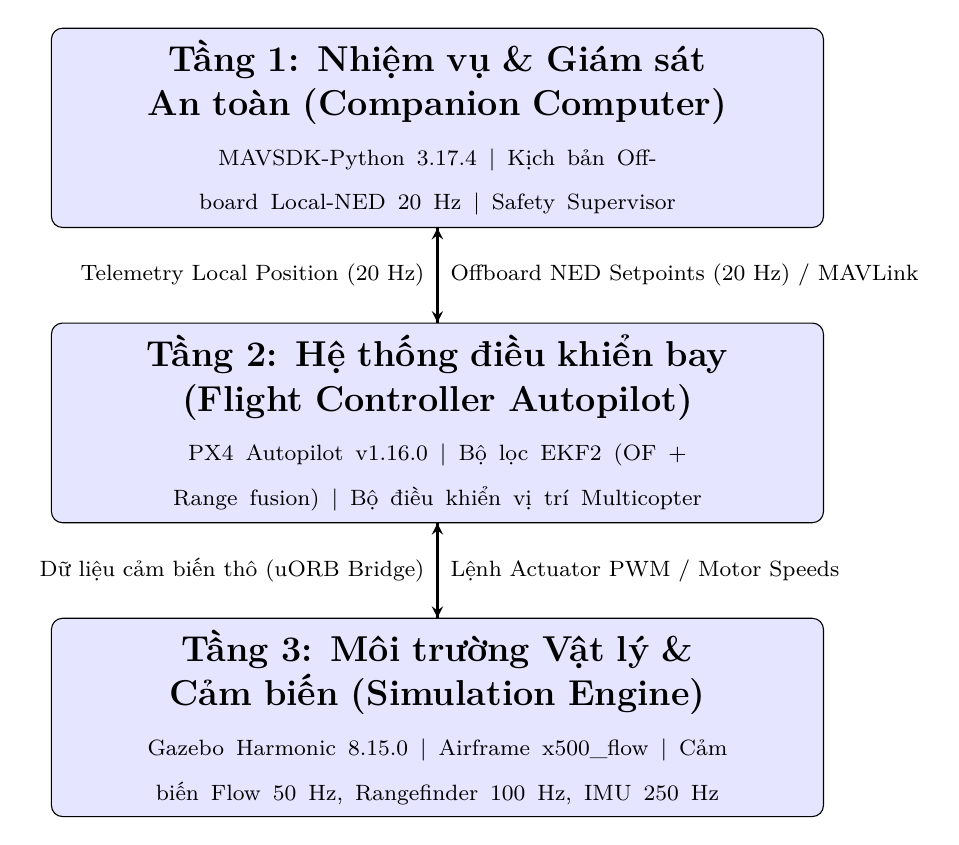
\begin{tikzpicture}[node distance=1.2cm, auto,
  block/.style={rectangle, draw, fill=blue!10, text width=9.5cm, text centered, rounded corners, minimum height=1.0cm},
  arrow/.style={thick, ->, >=stealth}]

  \node[block] (comp) {\textbf{Tầng 1: Nhiệm vụ \& Giám sát An toàn (Companion Computer)}\\[2pt]
    \footnotesize MAVSDK-Python 3.17.4 | Kịch bản Offboard Local-NED 20 Hz | Safety Supervisor};

  \node[block, below=of comp] (fc) {\textbf{Tầng 2: Hệ thống điều khiển bay (Flight Controller Autopilot)}\\[2pt]
    \footnotesize PX4 Autopilot v1.16.0 | Bộ lọc EKF2 (OF + Range fusion) | Bộ điều khiển vị trí Multicopter};

  \node[block, below=of fc] (sim) {\textbf{Tầng 3: Môi trường Vật lý \& Cảm biến (Simulation Engine)}\\[2pt]
    \footnotesize Gazebo Harmonic 8.15.0 | Airframe x500\_flow | Cảm biến Flow 50 Hz, Rangefinder 100 Hz, IMU 250 Hz};

  \draw[arrow] (comp) -- node[right, font=\footnotesize] {Offboard NED Setpoints (20 Hz) / MAVLink} (fc);
  \draw[arrow] (fc) -- node[left, font=\footnotesize] {Telemetry Local Position (20 Hz)} (comp);
  \draw[arrow] (fc) -- node[right, font=\footnotesize] {Lệnh Actuator PWM / Motor Speeds} (sim);
  \draw[arrow] (sim) -- node[left, font=\footnotesize] {Dữ liệu cảm biến thô (uORB Bridge)} (fc);
\end{tikzpicture}
\caption{Sơ đồ khối kiến trúc phân tầng hệ thống N01}\label{fig:arch}
\end{figure}

\subsection{Môi trường mô phỏng cô lập và Xử lý lỗi cấu hình}
Môi trường thực nghiệm được nhóm đóng gói trong Docker container\\
\code{n01-px4-sitl:v1.16.0} chạy trên nền Ubuntu 24.04 LTS, tích hợp Gazebo Harmonic và chế độ Offboard~\cite{source10,source11}. Phiên bản phần mềm được khóa cố định tại \code{sim/evidence/source-lock.json}:
\begin{itemize}
  \item PX4-Autopilot: Commit \code{6ea3539157ca358c70a515878b77077af7d4611d} (Tag v1.16.0).
  \item Gazebo Sim: Phiên bản 8.15.0 (Harmonic).
  \item Python 3.12.3 kèm MAVSDK-Python 3.17.4.
\end{itemize}

Khi thiết lập mô phỏng ban đầu, nhóm xử lý hai lỗi phát sinh trên PX4 v1.16 SITL:
\begin{enumerate}
  \item \textbf{Thiếu plugin OpticalFlowSystem:} Script khởi chạy Gazebo của PX4 v1.16 không tự nạp đường dẫn thư viện \code{libOpticalFlowSystem.so}, làm mất topic quang lưu. Nhóm xuất đường dẫn qua hai biến môi trường \code{GZ_SIM_SYSTEM_PLUGIN_PATH} và \code{GZ_SIM_SERVER_CONFIG_PATH} để nạp plugin đúng vị trí.
  \item \textbf{Hiện tượng trôi dạt do mặt sàn thiếu vân bề mặt (Featureless Ground):} Mô hình quang lưu dùng thuật toán bám góc Kanade--Lucas--Tomasi (KLT). Mặt sàn xám mặc định trong Gazebo có độ lệch chuẩn mức xám bằng 0 ($\text{std} = 0{,}0$), khiến thuật toán không thể trích xuất đặc trưng và trả về chất lượng $0/255$. Nhóm tạo mặt sàn có hoa văn bàn cờ đa tỉ lệ kết hợp nhiễu ngẫu nhiên kích thước $2048 \times 2048$ pixel (\code{textured_plane.png}, $\text{std} = 58{,}5$), đưa vào tệp mô tả thế giới \code{indoor_flow.sdf}. Hình~\ref{fig:textured_cam} là khung hình thực tế camera thu được.
\end{enumerate}

\begin{figure}[ht]
\centering

\includegraphics[width=0.45\linewidth]{figures/camera_frame_textured.png}
\caption{Khung hình thu từ camera quang lưu sau khi tích hợp vân bề mặt}\label{fig:textured_cam}
\end{figure}

\section{Kết quả thực nghiệm và Đo lường định lượng trên SITL (Gate G1)}

Hệ thống cần vượt qua cổng nghiệm thu mô phỏng Gate G1 với ba bài thử nghiệm độc lập. Số liệu được trích xuất từ tệp ULog và chuỗi thời gian CSV tại \code{sim/evidence/flight_logs/}.

\subsection{Thực nghiệm 1: Bay giữ vị trí tự động 30 giây (Hover Position Hold)}
Drone nhận lệnh cất cánh tự động bằng chế độ Offboard Local-NED, nâng độ cao lên $1{,}0\text{ m}$ ($z = -1{,}0\text{ m}$), giữ vị trí ổn định trong 30 giây và hạ cánh tự động. Kết quả đo đạc (Run ID \code{20261108_133915}) trình bày tại Bảng~\ref{tab:hover_metrics} và Hình~\ref{fig:hover_plot}. Cửa sổ 30 giây được đếm theo thời gian mô phỏng của PX4 (odometry), không theo đồng hồ thật, vì mô phỏng chạy dưới thời gian thực khi bật giao diện đồ họa. Sai số Ground Truth tính trong cửa sổ giữ vị trí, so với điểm Ground Truth lúc bắt đầu giữ vị trí, không so với gốc tọa độ để loại phần cất cánh.

\begingroup\tblfont
\begin{table}[ht]
\centering
\caption{Chỉ số thực nghiệm bay giữ vị trí 30 giây (Hover $1{,}0\text{ m}$)}\label{tab:hover_metrics}
\begin{tabularx}{\linewidth}{L{5.0cm}YYL{3.2cm}}
\toprule Chỉ số đánh giá & Giá trị thực nghiệm & Ngưỡng KPI đề tài & Kết luận\\\midrule
Thời gian giữ vị trí (thời gian mô phỏng) & $30{,}0\text{ s}$ & $30{,}0\text{ s}$ & Đạt\\
Sai số ngang cực đại ước lượng ($e_{\text{hold}}$) & $\mathbf{0{,}2336\text{ m}}$ & $\le 0{,}50\text{ m}$ & Đạt yêu cầu\\
\textbf{Sai số ngang cực đại Ground Truth ($e_{\text{GT}}$)} & $\mathbf{0{,}1300\text{ m}}$ & $\le \mathbf{0{,}50\text{ m}}$ & \textbf{Đạt chuẩn KPI}\\
RMSE lệch ước lượng so với Ground Truth & $0{,}0243\text{ m}$ & - & Ổn định tốt\\
Sai số độ cao so với mục tiêu $1{,}0\text{ m}$ & $\text{Max} = 0{,}1977\text{ m}$ ($\text{RMSE} = 0{,}0480\text{ m}$) & $[0{,}8\text{ m} \div 1{,}5\text{ m}]$ & Đạt\\
Tỷ lệ mẫu fuse Optical Flow thành công & $100\%$ ($1454 / 1454$ mẫu) & $\ge 80\%$ & Bộ lọc hội tụ tốt\\\bottomrule
\end{tabularx}
\end{table}
\endgroup

\begin{figure}[ht]
\centering
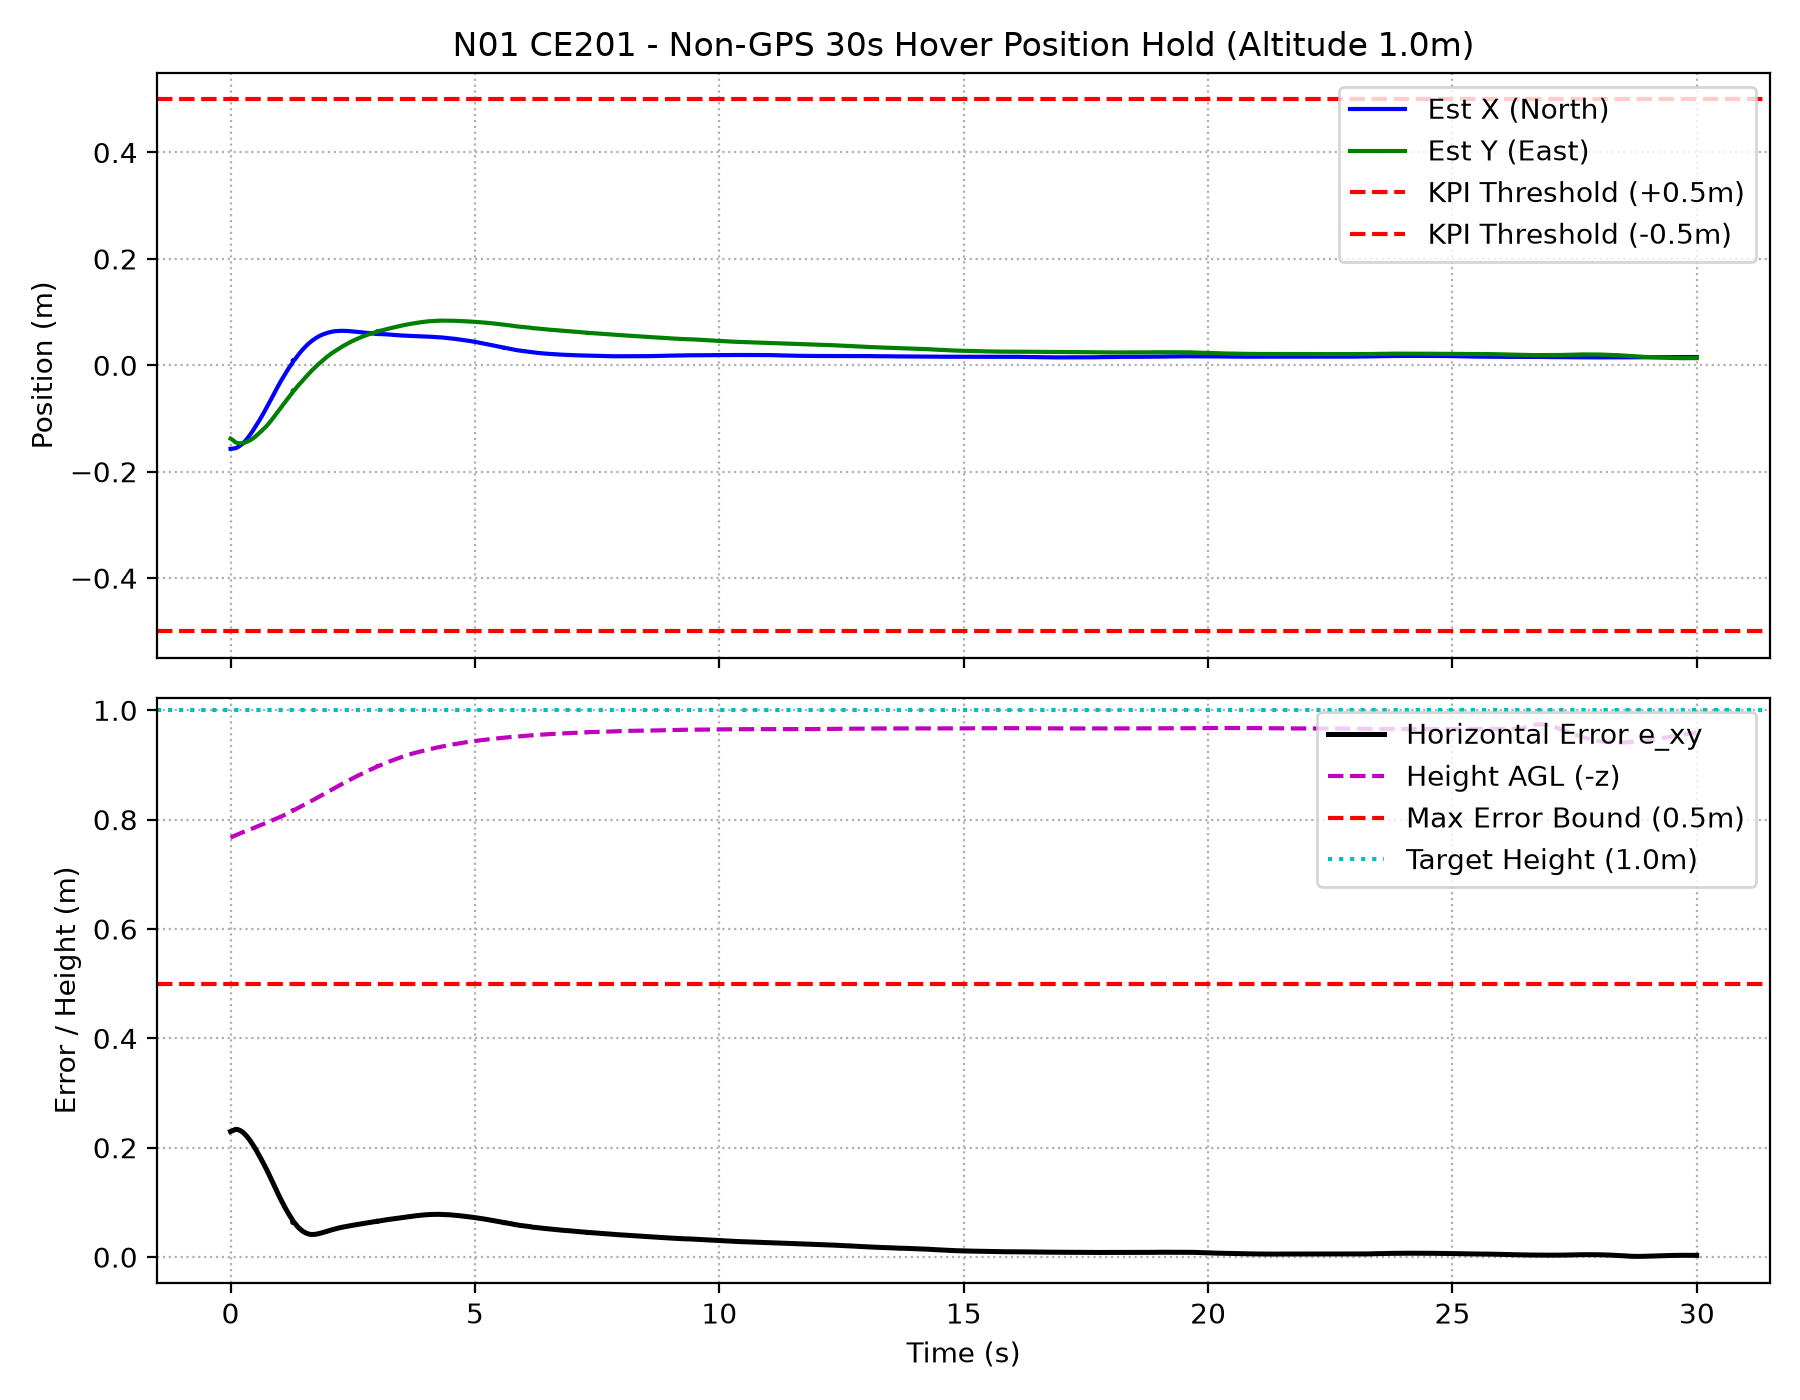
\includegraphics[width=0.88\linewidth]{figures/hover_plot.png}
\caption{Diễn biến tọa độ ngang và độ cao trong bài bay Hover 30 giây}\label{fig:hover_plot}
\end{figure}

\subsection{Thực nghiệm 2: Bay bám quỹ đạo hình vuông 2x2m (Square Trajectory)}
Drone thực hiện lộ trình bay qua 4 đỉnh: $W_0(0,0) \to W_1(2,0) \to W_2(2,2) \to W_3(0,2) \to W_4(0,0)\text{ m}$ ở độ cao $1{,}0\text{ m}$, vận tốc hành trình $0{,}25\text{ m/s}$ và dừng 3 giây tại mỗi đỉnh (Run ID \code{20261107_101837}). Kết quả chi tiết tại Bảng~\ref{tab:square_metrics} và Hình~\ref{fig:square_plot}. Video minh họa ghi lại một lần chạy lặp khác (Run ID \code{20261108_125334}, đủ $4/4$ đỉnh, sai số khép vòng Ground Truth $0{,}0647\text{ m}$); số liệu trong bảng lấy từ lần chạy gốc có log đầy đủ nêu trên.

\begingroup\tblfont
\begin{table}[ht]
\centering
\caption{Chỉ số thực nghiệm bay quỹ đạo hình vuông $2 \times 2\text{ m}$}\label{tab:square_metrics}
\begin{tabularx}{\linewidth}{L{3.6cm}L{3.2cm}L{4.8cm}Y}
\toprule Vị trí đỉnh / Chỉ số & Tọa độ danh định & Tọa độ thực tế đo được & Sai số vị trí\\\midrule
Đỉnh 1: $W_1$ (Bắc) & $(2{,}0\text{ m}, 0{,}0\text{ m})$ & $(2{,}020\text{ m}, 0{,}034\text{ m})$ & $\mathbf{0{,}0366\text{ m}}$ ($3{,}7\text{ cm}$)\\
Đỉnh 2: $W_2$ (Đông) & $(2{,}0\text{ m}, 2{,}0\text{ m})$ & $(2{,}006\text{ m}, 2{,}003\text{ m})$ & $\mathbf{0{,}0067\text{ m}}$ ($6{,}7\text{ mm}$)\\
Đỉnh 3: $W_3$ (Nam) & $(0{,}0\text{ m}, 2{,}0\text{ m})$ & $(-0{,}001\text{ m}, 2{,}009\text{ m})$ & $\mathbf{0{,}0091\text{ m}}$ ($9{,}1\text{ mm}$)\\
Đỉnh 4: $W_4$ (Về gốc) & $(0{,}0\text{ m}, 0{,}0\text{ m})$ & $(0{,}015\text{ m}, -0{,}036\text{ m})$ & $\mathbf{0{,}0347\text{ m}}$ ($3{,}5\text{ cm}$)\\
\textbf{Sai số khép vòng (Loop Closure GT)} & - & - & $\mathbf{0{,}0652\text{ m}}$ ($6{,}5\text{ cm}$)\\
Tổng thời gian bay & - & $45{,}41\text{ giây}$ (880 mẫu) & Hoàn thành $4/4$ đỉnh\\\bottomrule
\end{tabularx}
\end{table}
\endgroup

\begin{figure}[ht]
\centering
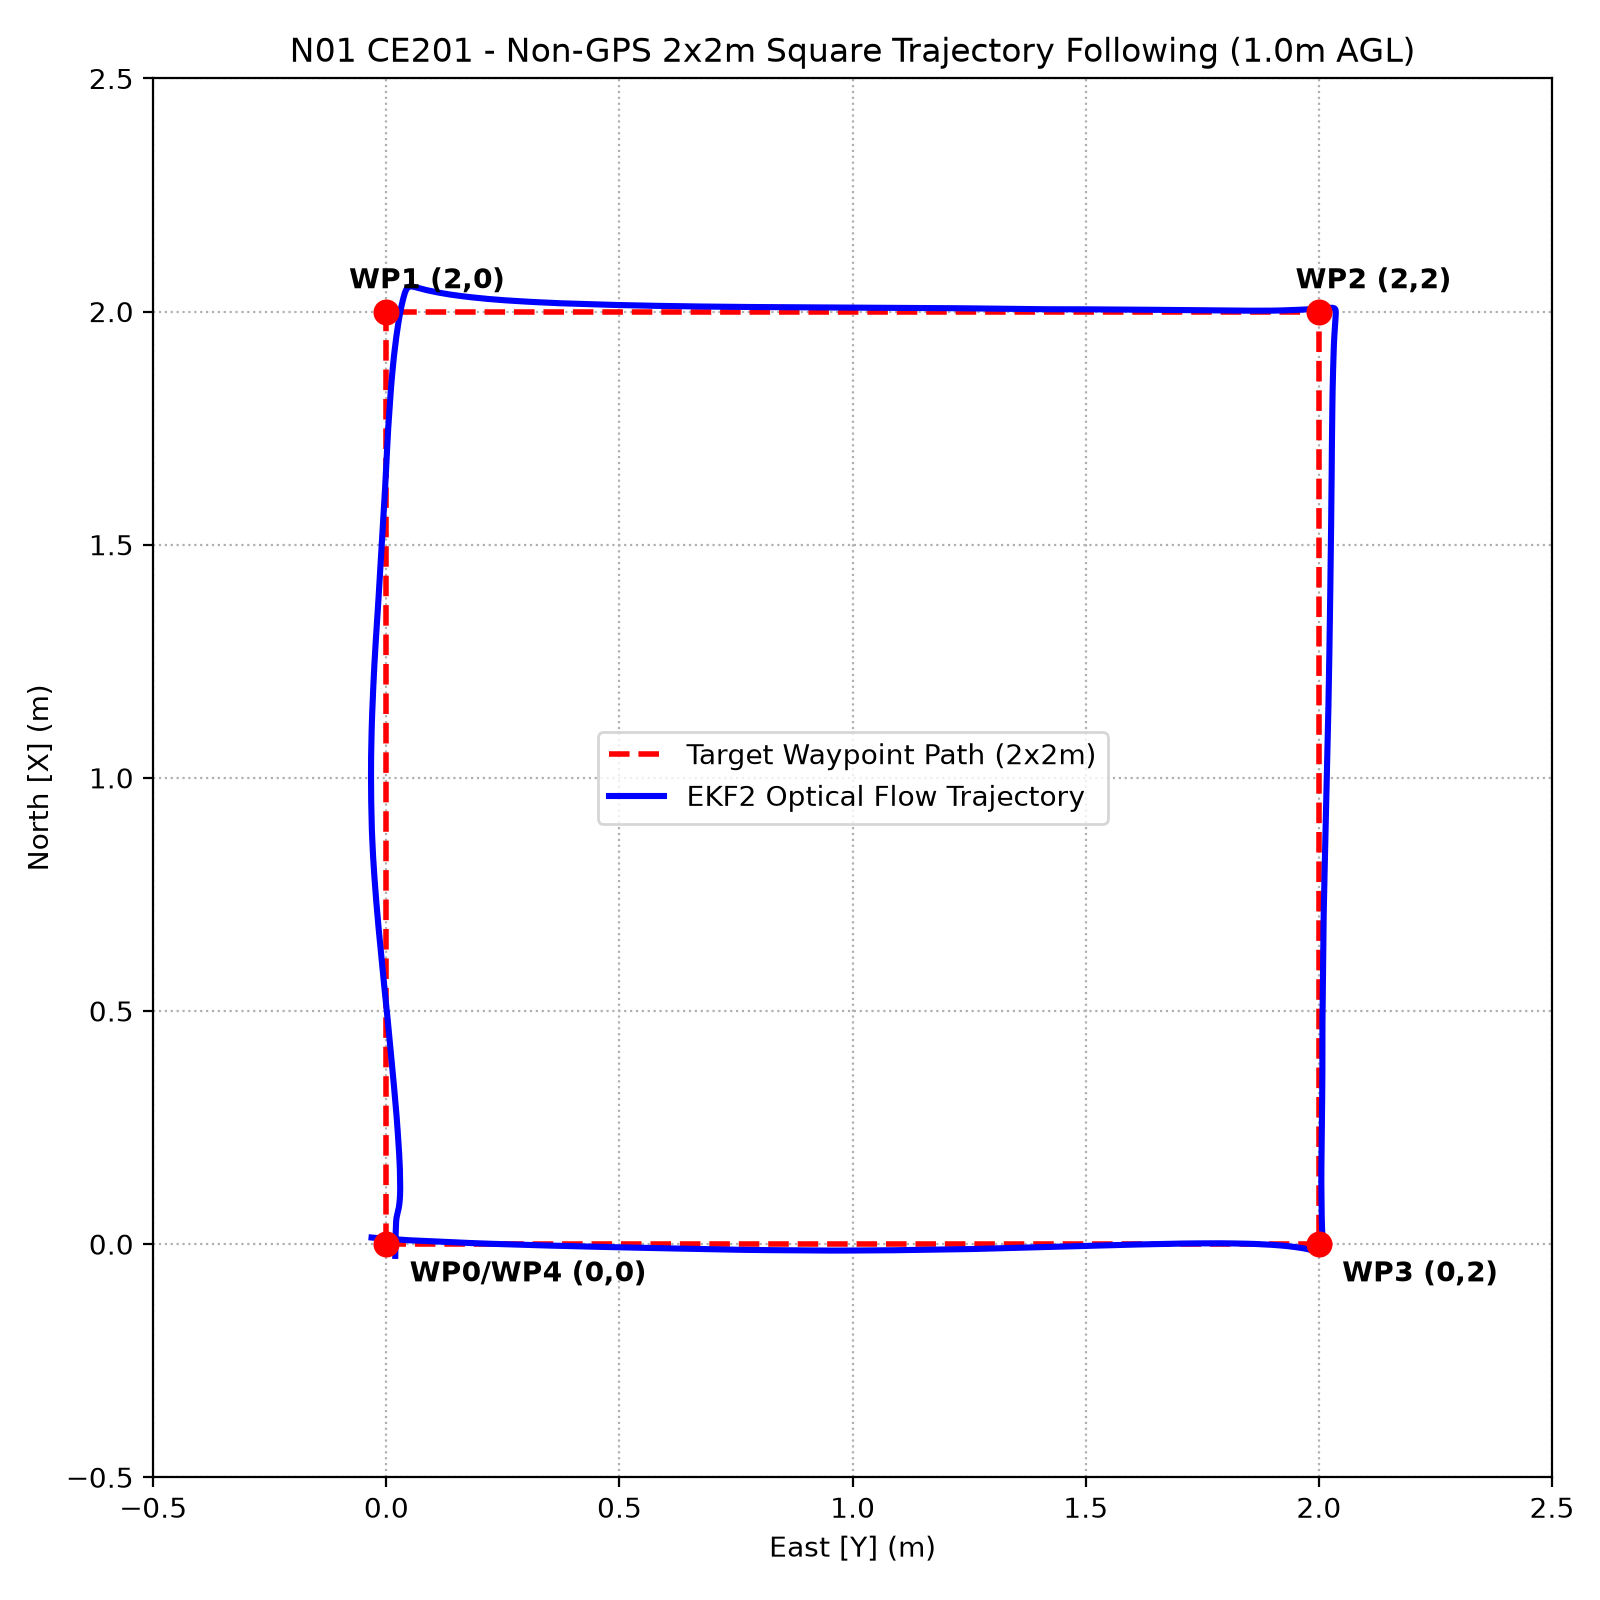
\includegraphics[width=0.65\linewidth]{figures/square_plot.png}
\caption{Quỹ đạo 2D mặt phẳng ngang (East-North) bài bay hình vuông $2 \times 2\text{ m}$}\label{fig:square_plot}
\end{figure}

\subsection{Thực nghiệm 3: Kiểm thử an toàn và Xử lý sự cố (Fault Injection)}
Để kiểm tra khả năng vận hành an toàn theo chuẩn CĐR PLO4 của học phần CE201, kịch bản \code{src/test_fault_injection.py} mô phỏng sự cố mất liên lạc hoàn toàn với Companion Computer khi drone đang giữ vị trí ở độ cao $1{,}0\text{ m}$ (ngắt tiến trình \code{mavsdk_server}).
\begin{itemize}
  \item \textbf{Phát hiện sự cố:} Sau thời gian chờ $1{,}0\text{ s}$ (\code{COM_OF_LOSS_T=1.0}), PX4 nhận diện mất luồng setpoint Offboard.
  \item \textbf{Kích hoạt Failsafe:} Với cấu hình tham số \code{COM_OBL_RC_ACT=4}, autopilot tự động chuyển sang chế độ \textbf{AUTO\_LAND} (\code{nav_state=18}), không để drone trôi dạt tự do.
  \item \textbf{Hạ cánh và ngắt động cơ:} Drone hạ cánh có kiểm soát xuống mặt sàn với vận tốc tiếp đất $v_z \approx -0{,}02\text{ m/s}$. Bộ phát hiện tiếp đất (Land Detector) xác nhận chạm sàn và tự động ngắt động cơ (\textbf{DISARMED}) ở giây thứ $13{,}6$ (Run ID \code{20261107_103243}).
\end{itemize}

Kết quả cho thấy hệ thống đáp ứng đầy đủ các tiêu chí nghiệm thu Gate G1 SITL.

\section{Đánh giá độ lệch phần cứng và Kế hoạch triển khai mốc M3}

\subsection{Phân tích độ lệch giữa mô phỏng và phần cứng thực tế}
Theo thông báo của GVHD ngày 23/10/2026~\cite{source1}, phòng Lab dự kiến cho mượn 1 mạch điều khiển bay STM32F405 để chuẩn bị thử nghiệm thực tế. Nhóm nhận diện các điểm khác biệt kỹ thuật (hardware gap):
\begin{itemize}
  \item Mô phỏng hiện tại sử dụng \textbf{PX4 v1.16} (EKF2) và MAVSDK.
  \item Vi điều khiển STM32F405 có dung lượng bộ nhớ flash giới hạn ($1\text{ MB}$), thường chạy firmware \textbf{ArduPilot} (Copter EKF3) hoặc bản PX4 rút gọn.
\end{itemize}
Do đó, mã nguồn tầng Companion Computer giao tiếp qua giao thức MAVLink 2.0 chuẩn và thư viện MAVSDK. Cách tiếp cận này giúp kịch bản điều khiển có thể tái sử dụng nếu cần chuyển đổi sang ArduPilot ở các mốc sau.

\subsection{Kế hoạch triển khai sau mốc M2 (Tuần 7--9)}
\begin{enumerate}
  \item \textbf{Gate G2 -- Thử nghiệm bàn không cánh (Bench Test):} Kiểm tra cảm biến quang lưu PMW3901 và cảm biến khoảng cách VL53L1X trên bàn thử, kiểm tra dấu vận tốc, chất lượng đo và khả năng ngắt khẩn cấp bằng RC trước khi lắp cánh.
  \item \textbf{Đóng gói Prototype M3 (Hạn 30/11/2026):} Tích hợp luồng bay chính, thống kê độ trôi tích lũy và đề xuất phương án bù trôi trong báo cáo M3.
\end{enumerate}

\section{Kết luận}
Báo cáo mốc M2 đã hoàn thành các mục tiêu theo đề cương học phần CE201:
\begin{itemize}
  \item Luận giải cơ sở kỹ thuật của giải pháp định vị trong nhà bằng Optical Flow kết hợp Rangefinder và bộ lọc EKF2.
  \item Xây dựng môi trường mô phỏng cô lập trên nền Docker, xử lý lỗi thiếu plugin quang lưu và bổ sung mặt sàn có hoa văn để thuật toán KLT hoạt động ổn định.
  \item Kiểm chứng định lượng ba bài thử nghiệm cốt lõi trên SITL: giữ vị trí 30 giây đạt sai số Ground Truth cực đại $0{,}13\text{ m} \le 0{,}50\text{ m}$ (đáp ứng KPI đề tài); bay quỹ đạo hình vuông $2 \times 2\text{ m}$ qua 4 đỉnh với sai số khép vòng $6{,}5\text{ cm}$; và kiểm thử tiêm lỗi mất kết nối máy tính đồng hành, kích hoạt failsafe tự động hạ cánh và ngắt động cơ an toàn.
\end{itemize}

\begingroup\setstretch{1.0}\normalsize\raggedright
\begin{thebibliography}{99}
\bibitem{source1} N. D. X. Bách, “Đồ án 1 -- Đồ án 2, HK1 2026--2027: Mô tả đề tài và kế hoạch thực hiện,” Khoa KTMT, Trường ĐH Công nghệ Thông tin, ĐHQG-HCM, 09/2026.
\bibitem{source2} N. Gageik, M. Strohmeier, and S. Montenegro, “An autonomous UAV with an optical flow sensor for positioning and navigation,” \textit{Int. J. Adv. Robot. Syst.}, vol. 10, no. 10, 2013, doi: \href{https://doi.org/10.5772/56813}{10.5772/56813}.
\bibitem{source3} V. Grabe, H. H. Bülthoff, D. Scaramuzza, and P. R. Giordano, “Nonlinear ego-motion estimation from optical flow for online control of a quadrotor UAV,” \textit{Int. J. Robot. Res.}, vol. 34, no. 8, pp. 1114--1135, 2015, doi: \href{https://doi.org/10.1177/0278364915578646}{10.1177/0278364915578646}.
\bibitem{source4} J. R. Meza-Ibarra, J. Martínez-Ulloa, L. A. Moreno-Pacheco, and H. Rodríguez-Cortés, “A sensor fusion approach to observe quadrotor velocity,” \textit{Sensors}, vol. 24, no. 11, art. 3605, 2024, doi: \href{https://doi.org/10.3390/s24113605}{10.3390/s24113605}.
\bibitem{source5} T. Qin, P. Li, and S. Shen, “VINS-Mono: A robust and versatile monocular visual-inertial state estimator,” \textit{IEEE Trans. Robot.}, vol. 34, no. 4, pp. 1004--1020, 2018, doi: \href{https://doi.org/10.1109/TRO.2018.2853729}{10.1109/TRO.2018.2853729}.
\bibitem{source6} R. Wang, D. Zou, C. Xu, L. Pei, P. Liu, and W. Yu, “An aerodynamic model-aided state estimator for multi-rotor UAVs,” in \textit{Proc. IEEE/RSJ IROS}, 2017, pp. 2164--2170, doi: \href{https://doi.org/10.1109/IROS.2017.8206034}{10.1109/IROS.2017.8206034}.
\bibitem{source7} M.-T. Nguyen \textit{et al.}, “Stabilzation position of quadcopter using vision-based corner detector from top-down footage of camera,” \textit{J. Tech. Educ. Sci.}, no. 71A, pp. 18--27, 2022, doi: \href{https://doi.org/10.54644/jte.71A.2022.1132}{10.54644/jte.71A.2022.1132}.
\bibitem{source8} PX4 Development Team, “Optical Flow,” \textit{PX4 User Guide}, 2026. [Online]. Available: \url{https://docs.px4.io/main/en/sensor/optical_flow.html}.
\bibitem{source9} PX4 Development Team, “Using PX4's Navigation Filter (EKF2),” \textit{PX4 User Guide}, 2026. [Online]. Available: \url{https://docs.px4.io/main/en/advanced_config/tuning_the_ecl_ekf.html}.
\bibitem{source10} PX4 Development Team, “Gazebo Simulation,” \textit{PX4 User Guide}, 2026. [Online]. Available: \url{https://docs.px4.io/main/en/sim_gazebo_gz/}.
\bibitem{source11} PX4 Development Team, “Offboard Mode,” \textit{PX4 User Guide}, 2026. [Online]. Available: \url{https://docs.px4.io/main/en/flight_modes/offboard.html}.
\end{thebibliography}
\endgroup

\end{document}
